% GNUPLOT: LaTeX picture with Postscript
\begingroup
  \makeatletter
  \providecommand\color[2][]{%
    \GenericError{(gnuplot) \space\space\space\@spaces}{%
      Package color not loaded in conjunction with
      terminal option `colourtext'%
    }{See the gnuplot documentation for explanation.%
    }{Either use 'blacktext' in gnuplot or load the package
      color.sty in LaTeX.}%
    \renewcommand\color[2][]{}%
  }%
  \providecommand\includegraphics[2][]{%
    \GenericError{(gnuplot) \space\space\space\@spaces}{%
      Package graphicx or graphics not loaded%
    }{See the gnuplot documentation for explanation.%
    }{The gnuplot epslatex terminal needs graphicx.sty or graphics.sty.}%
    \renewcommand\includegraphics[2][]{}%
  }%
  \providecommand\rotatebox[2]{#2}%
  \@ifundefined{ifGPcolor}{%
    \newif\ifGPcolor
    \GPcolorfalse
  }{}%
  \@ifundefined{ifGPblacktext}{%
    \newif\ifGPblacktext
    \GPblacktexttrue
  }{}%
  % define a \g@addto@macro without @ in the name:
  \let\gplgaddtomacro\g@addto@macro
  % define empty templates for all commands taking text:
  \gdef\gplbacktext{}%
  \gdef\gplfronttext{}%
  \makeatother
  \ifGPblacktext
    % no textcolor at all
    \def\colorrgb#1{}%
    \def\colorgray#1{}%
  \else
    % gray or color?
    \ifGPcolor
      \def\colorrgb#1{\color[rgb]{#1}}%
      \def\colorgray#1{\color[gray]{#1}}%
      \expandafter\def\csname LTw\endcsname{\color{white}}%
      \expandafter\def\csname LTb\endcsname{\color{black}}%
      \expandafter\def\csname LTa\endcsname{\color{black}}%
      \expandafter\def\csname LT0\endcsname{\color[rgb]{1,0,0}}%
      \expandafter\def\csname LT1\endcsname{\color[rgb]{0,1,0}}%
      \expandafter\def\csname LT2\endcsname{\color[rgb]{0,0,1}}%
      \expandafter\def\csname LT3\endcsname{\color[rgb]{1,0,1}}%
      \expandafter\def\csname LT4\endcsname{\color[rgb]{0,1,1}}%
      \expandafter\def\csname LT5\endcsname{\color[rgb]{1,1,0}}%
      \expandafter\def\csname LT6\endcsname{\color[rgb]{0,0,0}}%
      \expandafter\def\csname LT7\endcsname{\color[rgb]{1,0.3,0}}%
      \expandafter\def\csname LT8\endcsname{\color[rgb]{0.5,0.5,0.5}}%
    \else
      % gray
      \def\colorrgb#1{\color{black}}%
      \def\colorgray#1{\color[gray]{#1}}%
      \expandafter\def\csname LTw\endcsname{\color{white}}%
      \expandafter\def\csname LTb\endcsname{\color{black}}%
      \expandafter\def\csname LTa\endcsname{\color{black}}%
      \expandafter\def\csname LT0\endcsname{\color{black}}%
      \expandafter\def\csname LT1\endcsname{\color{black}}%
      \expandafter\def\csname LT2\endcsname{\color{black}}%
      \expandafter\def\csname LT3\endcsname{\color{black}}%
      \expandafter\def\csname LT4\endcsname{\color{black}}%
      \expandafter\def\csname LT5\endcsname{\color{black}}%
      \expandafter\def\csname LT6\endcsname{\color{black}}%
      \expandafter\def\csname LT7\endcsname{\color{black}}%
      \expandafter\def\csname LT8\endcsname{\color{black}}%
    \fi
  \fi
  \setlength{\unitlength}{0.0500bp}%
  \begin{picture}(15306.00,10204.00)%
    \gplgaddtomacro\gplbacktext{%
      \csname LTb\endcsname%
      \put(814,704){\makebox(0,0)[r]{\strut{} 0}}%
      \put(814,2177){\makebox(0,0)[r]{\strut{} 10}}%
      \put(814,3650){\makebox(0,0)[r]{\strut{} 20}}%
      \put(814,5124){\makebox(0,0)[r]{\strut{} 30}}%
      \put(814,6597){\makebox(0,0)[r]{\strut{} 40}}%
      \put(814,8070){\makebox(0,0)[r]{\strut{} 50}}%
      \put(814,9543){\makebox(0,0)[r]{\strut{} 60}}%
      \put(946,484){\makebox(0,0){\strut{} 0}}%
      \put(2497,484){\makebox(0,0){\strut{} 0.1}}%
      \put(4049,484){\makebox(0,0){\strut{} 0.2}}%
      \put(5600,484){\makebox(0,0){\strut{} 0.3}}%
      \put(7152,484){\makebox(0,0){\strut{} 0.4}}%
      \put(8703,484){\makebox(0,0){\strut{} 0.5}}%
      \put(10255,484){\makebox(0,0){\strut{} 0.6}}%
      \put(11806,484){\makebox(0,0){\strut{} 0.7}}%
      \put(13358,484){\makebox(0,0){\strut{} 0.8}}%
      \put(14909,484){\makebox(0,0){\strut{} 0.9}}%
      \put(176,5123){\rotatebox{-270}{\makebox(0,0){\strut{}$I$ [mA]}}}%
      \put(7927,154){\makebox(0,0){\strut{}$U$ [V]}}%
      \put(7927,9873){\makebox(0,0){\strut{}Plot 3: Diodenkennlinie}}%
      \put(1923,1058){\makebox(0,0)[l]{\strut{}Gestrichelte Linie: 1 mA}}%
      \put(1923,8659){\makebox(0,0)[l]{\strut{}Fit gegen Shockley-Gleichung}}%
      \put(1923,8439){\makebox(0,0)[l]{\strut{}Lineare Regression durch letzte 5 Messwerte zur}}%
      \put(1923,8219){\makebox(0,0)[l]{\strut{}Bestimmung der Schwellenspannung}}%
      \put(1923,7999){\makebox(0,0)[l]{\strut{}}}%
      \put(1923,7779){\makebox(0,0)[l]{\strut{}Fitgleichung $I(U) = -I_0 + \frac{U}{R_D}$}}%
      \put(1923,6891){\makebox(0,0)[l]{\strut{}$I_0 = \num{714.7+-436.6}\,\text{mA}$}}%
      \put(1923,6626){\makebox(0,0)[l]{\strut{}$1/R_D = \num{987.5+-580.4} /k\Omega$}}%
    }%
    \gplgaddtomacro\gplfronttext{%
    }%
    \gplbacktext
    \put(0,0){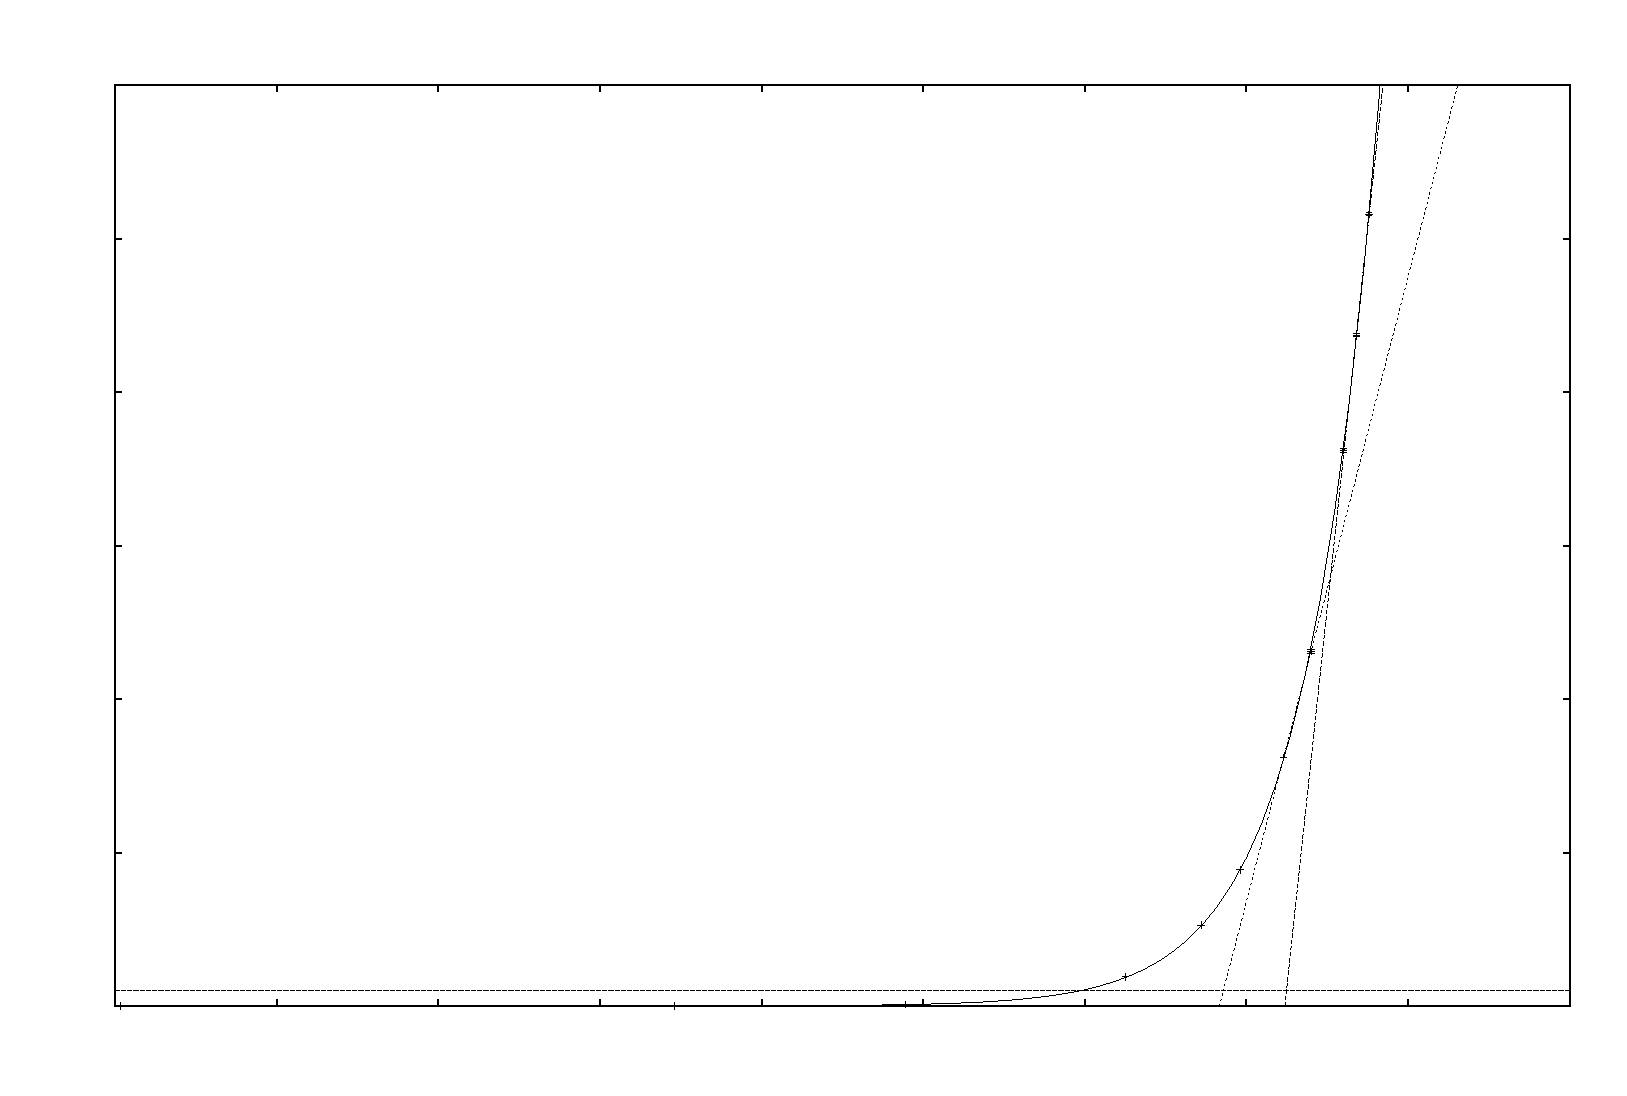
\includegraphics{plot-1}}%
    \gplfronttext
  \end{picture}%
\endgroup
